\section{Experiments}
\label{sec:experiments}
We evaluate \acro\ and justify our design choices on real point clouds, using \emph{3DMatch}~\cite{zeng20163dmatch} and \emph{3DLoMatch} (\cref{sec:3DMatch}). Additionally, we compare \acro\ to direct registration methods on the synthetic, object-centric \emph{ModelNet40}~\cite{wu2015ModelNet} (\cref{sec:model_net}) and evaluate it on large outdoor scenes using odometryKITTI~\cite{geiger2012kitti} (\cref{sec:kitti}). More details about the datasets and evaluation metrics are available in the Appndix. Qualitative results are shown in Fig.~\ref{fig:3DMatch_qualitative}.

\begin{figure}[t]
    \centering
    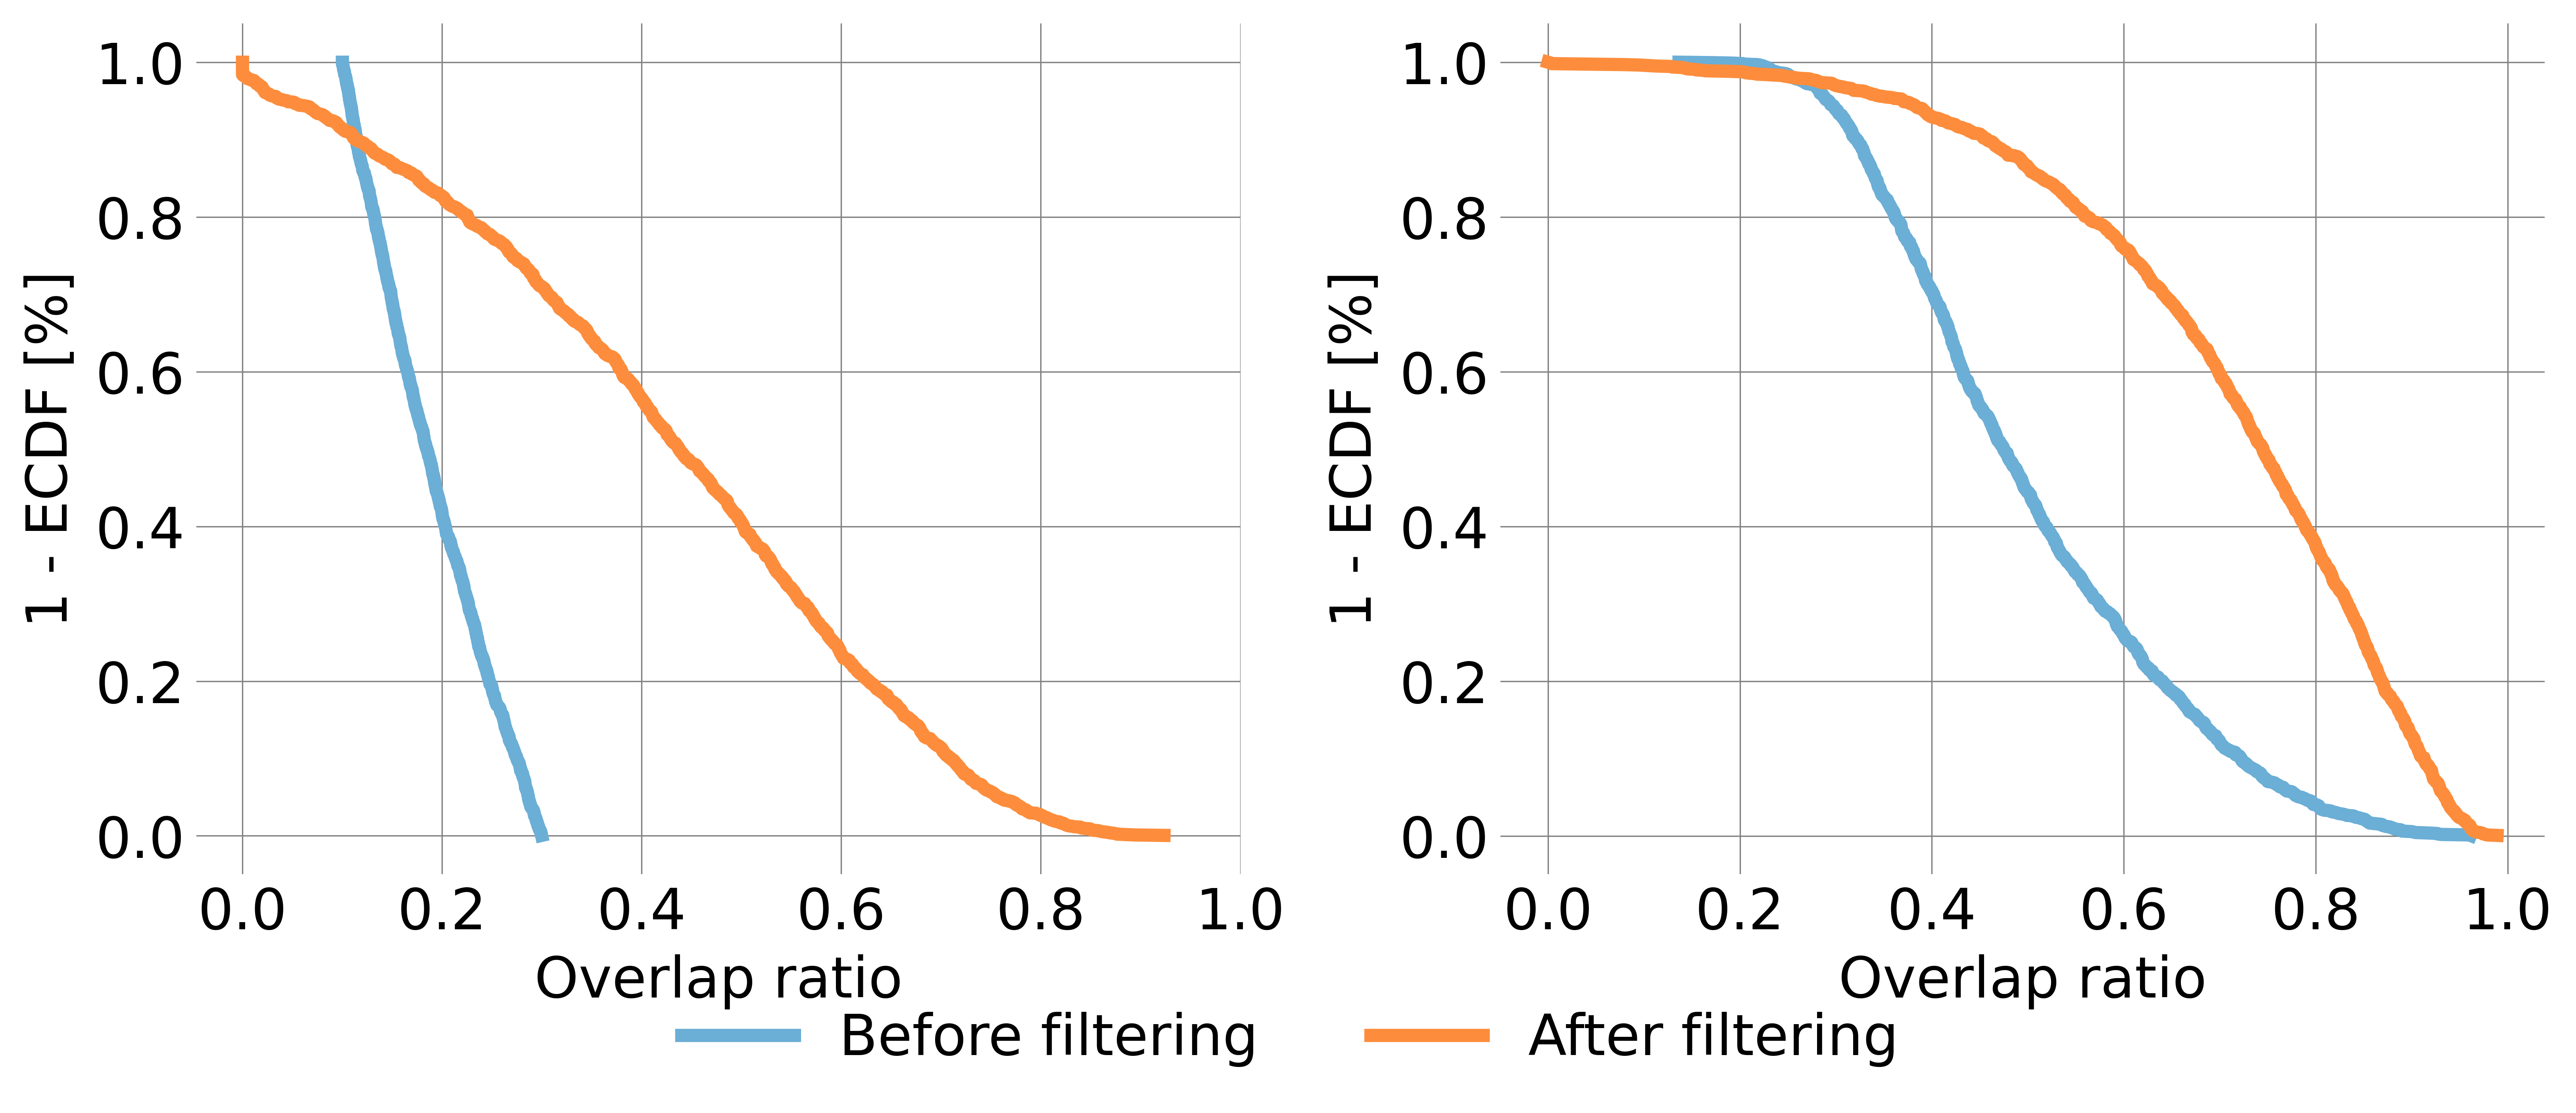
\includegraphics[width=0.8\columnwidth]{figures/images/improve_overlap.png}
    \caption{Distribution of the relative overlap ratio before and after filtering the points with the inferred overlap scores, \textit{3DLoMatch} (left) and \textit{3DMatch} (right).}
    \label{fig:imp_overlap}
    
\end{figure}
\subsection{3DMatch}
\label{sec:3DMatch}
\paragraph{Dataset}
~\cite{zeng20163dmatch} is a collection of 62 scenes, from which we use 46 scenes for training, 8 scenes for validation and 8 for testing. Official \emph{3DMatch} dataset considers only scan pairs with \textgreater30\% overlap. Here, we add its counterpart in which we consider only scan pairs with overlaps between 10 and 30\% and call this collection \textit{3DLoMatch}\footnote{Due to a bug in the official implementation of the overlap computation for \emph{3DMatch}, a few (\textless7\%) scan pairs are included in both datasets.}. 

\paragraph{Metrics}
Our main metric, corresponding to the actual aim of point cloud registration, is \emph{Registration Recall~(RR)}, i.e., the fraction of scan pairs for which the correct transformation parameters are found with RANSAC.
Following the literature~\cite{zeng20163dmatch, gojcic2018learned, Choy2019FCGF}, we also report 
\emph{Feature Match Recall~(FMR)}, defined as the fraction of pairs 
that have \textgreater5\% "inlier" matches with \textless10~cm residual under the ground truth transformation (without checking if the transformation can be recovered from those matches), and \emph{Inlier Ratio~(IR)}, the fraction of correct correspondences among the putative matches. Additionally, we use empirical cumulative distribution functions (ECDF) to evaluate the relative overlap ratio. At a specific overlap value, the $(1\!-\!\text{ECDF})$ curve shows the fraction of fragment pairs that have relative overlap greater or equal to that value.

\paragraph{Relative overlap ratio}
We first evaluate if \acro\ achieves its goal to focus on the overlap. We discard points with a predicted overlap score
$\mathbf{o}_i\!<\!0.5$, compute the overlap ratio, and compare it to the one of the original scans.
Fig.~\ref{fig:imp_overlap} shows that more than half ($71\%$) of the low-overlap pairs are pushed over the 30\% threshold that prior works considered the lower limit for registration. On average, discarding points with low overlap scores almost doubles the overlap in \emph{3DLoMatch} ($133\%$ increase).
Notably, it also increases the overlap in standard \emph{3DMatch} by, on average, \textgreater50\%.

\begin{figure}[t]
    \centering
    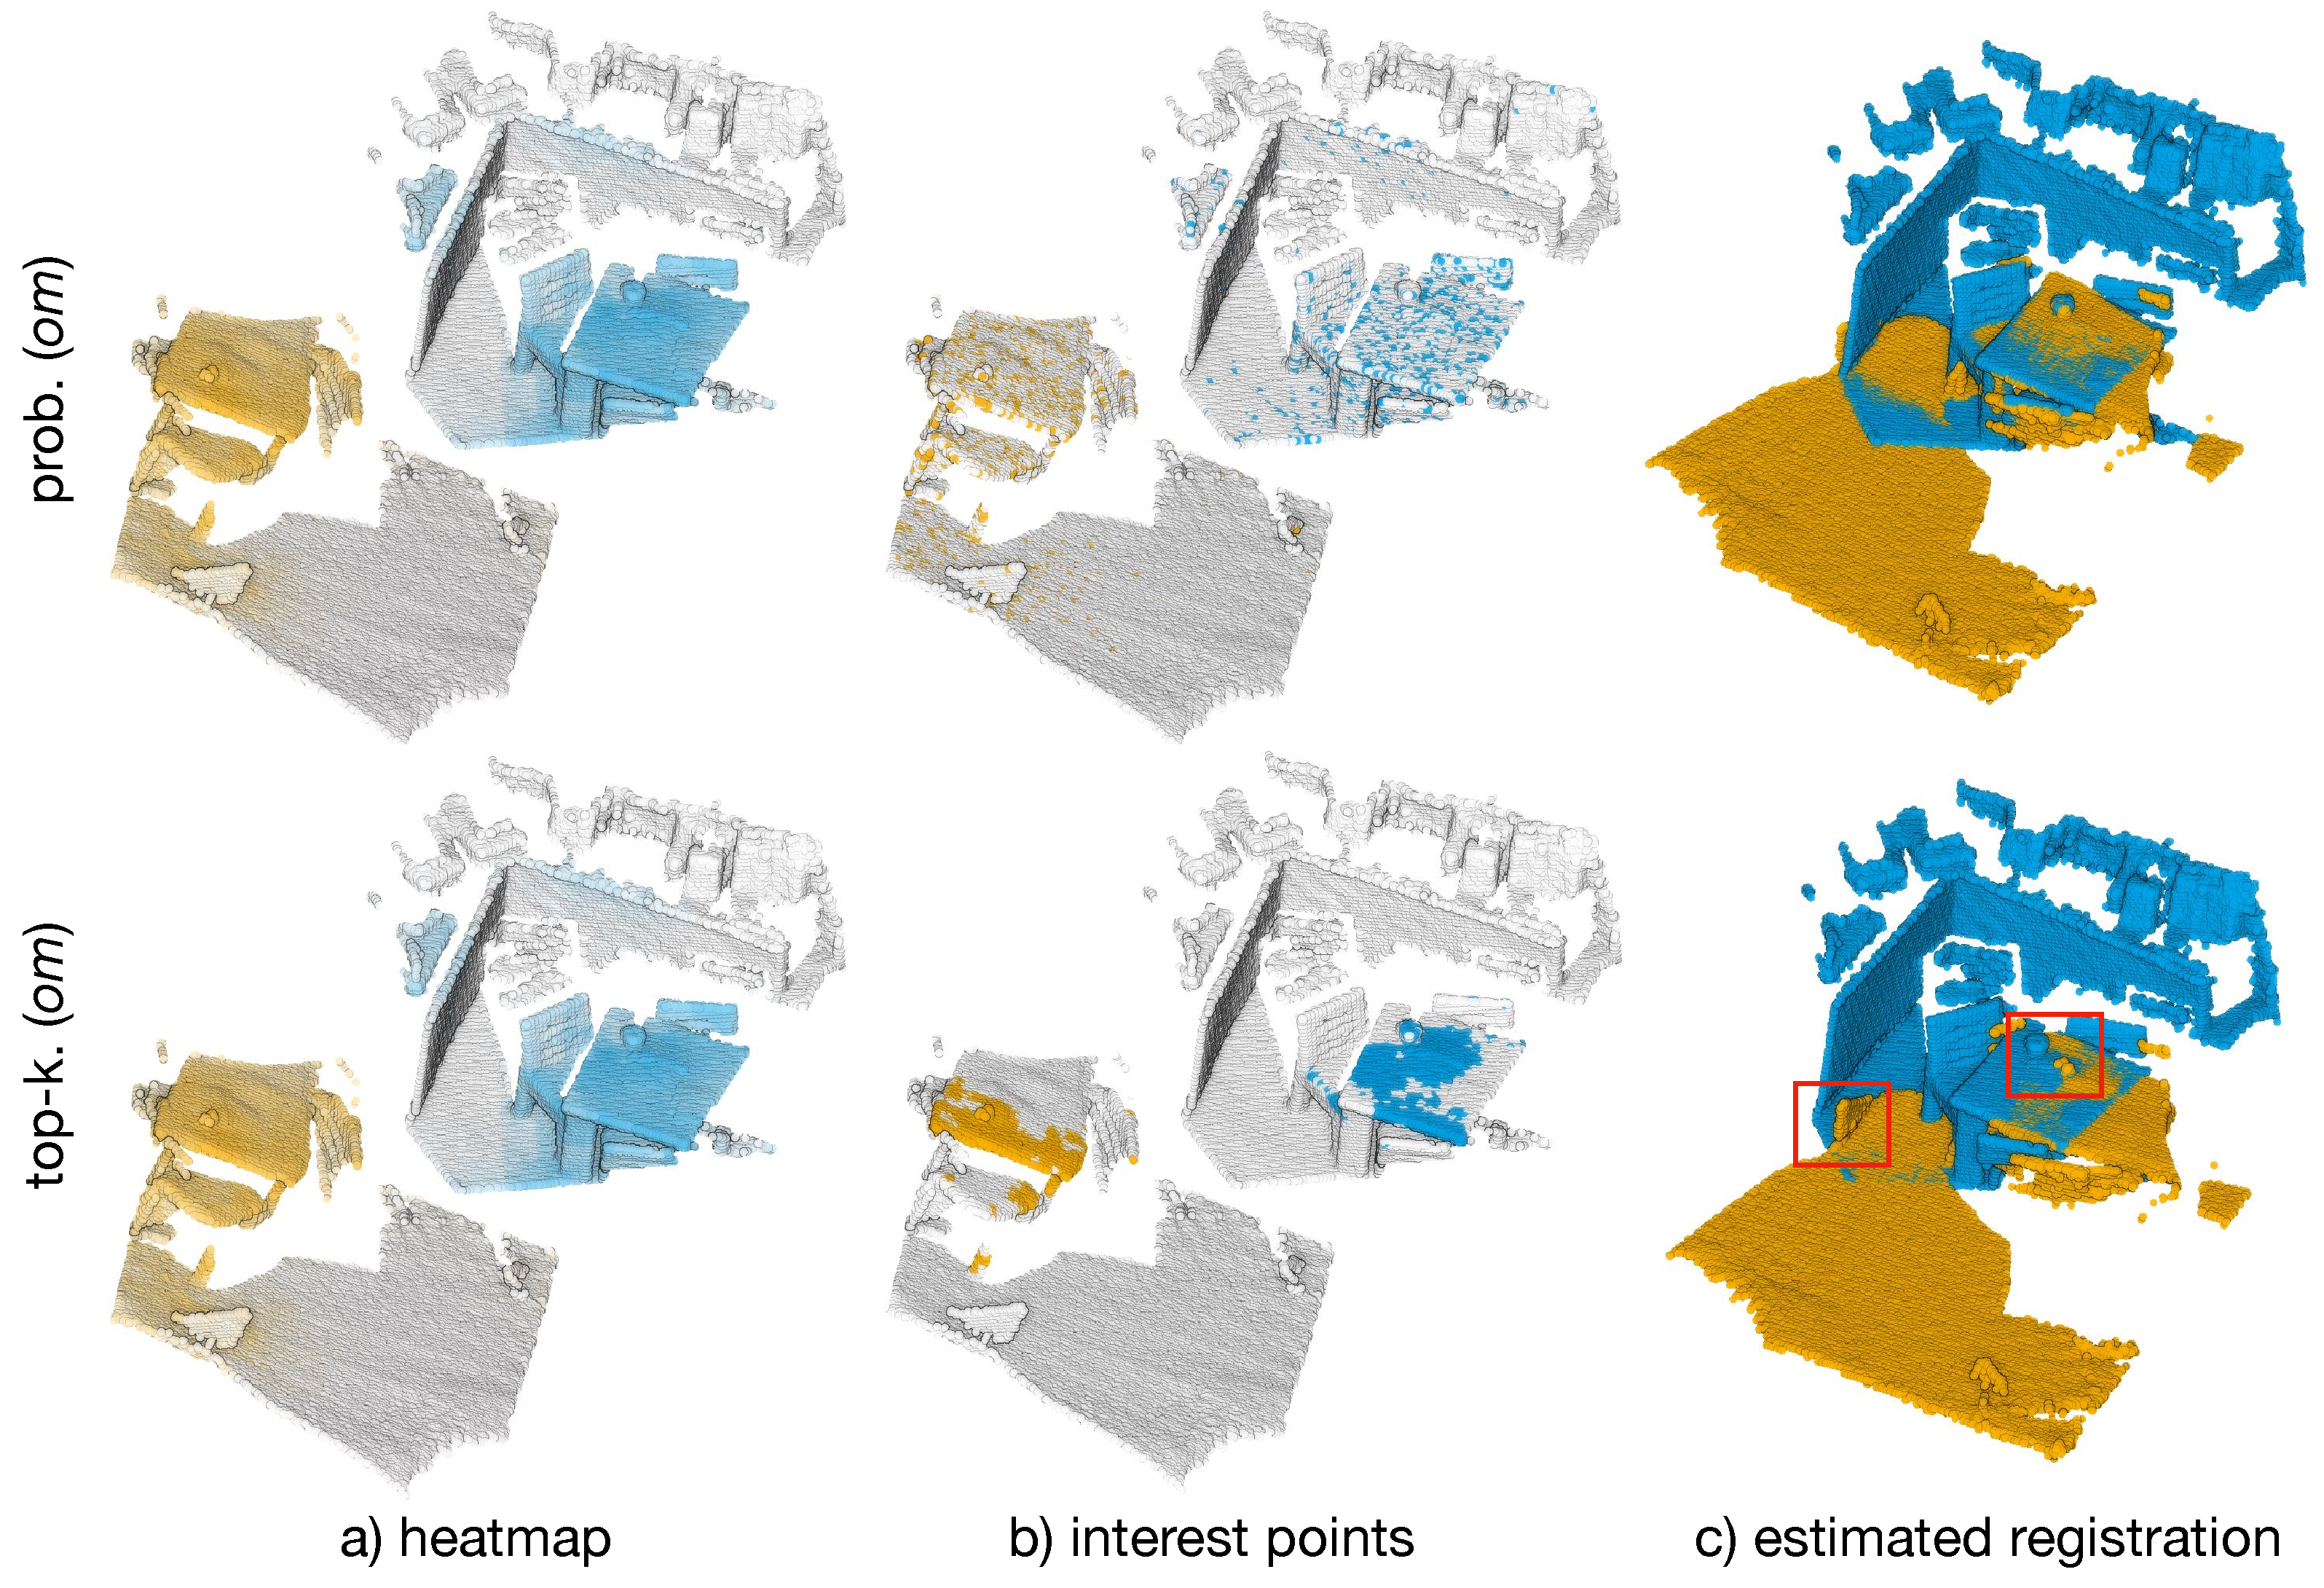
\includegraphics[width=\columnwidth]{figures/images/demo_sampling.pdf}
    \caption{\emph{Top-k ($om$)} sampling yields clustered interest points, whereas the points obtained with \emph{prob. ($om$)} sampling are more scattered and thus enable a more robust estimation of the transformation parameters.}
    \label{fig:sampling}
\end{figure}
\begin{table}[t]
    \setlength{\tabcolsep}{6pt}
    \renewcommand{\arraystretch}{1.2}
	\centering
	\resizebox{\columnwidth}{!}{
    \begin{tabular}{lccccc|ccccc}
			\toprule
			& \multicolumn{5}{c|}{\textit{3DMatch}} & \multicolumn{5}{c}{\textit{3DLoMatch}} \\

			\# Samples (k) & 5000 & 2500 & 1000 & 500 & 250 & 5000 & 2500 & 1000 & 500 & 250 \\
			\midrule
	

			& \multicolumn{10}{c}{\textit{Inlier ratio (\%)}} \\
			\midrule
			\emph{rand} & 51.6 & 49.5 & 44.5 & 38.9 & 32.1 & 20.4 & 19.2 & 16.8 & 14.3 & 11.5 \\
 			\emph{top-k ($om$)} & \textbf{68.4} & \textbf{73.8} & \textbf{77.6} & \textbf{78.6} & \textbf{78.7} & \textbf{33.7} & \textbf{39.9} & \textbf{44.9} & \textbf{47.0} & \textbf{47.7} \\
 			\emph{prob. ($om$)} & \underline{58.0} & \underline{58.4} & \underline{57.1} & \underline{54.1} & \underline{49.3} & \underline{26.7} & \underline{28.1} & \underline{28.3} & \underline{27.5} & \underline{25.8} \\

			\midrule
			& \multicolumn{10}{c}{\textit{Registration Recall (\%)}} \\
			\midrule
			\emph{rand} & 86.0 & 84.8 & \underline{84.7} & \underline{81.7} & \underline{75.3} & 43.3 & 45.3 & 40.4 & 35.9 & 28.0 \\
 			\emph{top-k ($om$)} & \underline{88.9} & \underline{87.4} & 82.0 & 75.6 & 64.0 & \underline{58.5} & \underline{57.8} & \underline{53.1} & \underline{44.9} & \underline{35.9} \\
 			\emph{prob. ($om$)} & \textbf{89.0} & \textbf{89.9} & \textbf{90.6} & \textbf{88.5} & \textbf{86.6} & \textbf{59.8} & \textbf{61.2} & \textbf{62.4} & \textbf{60.8} & \textbf{58.1}  \\
			\bottomrule
			
	\end{tabular}
	}
	\caption{%
	Performance of \acro\ with different interest point sampling strategies; $om$ denotes the product of overlap score and matchability score.
	}
	\label{tab:3DMatch_sampling}
    
\end{table}
\begin{figure}[t]
    \centering
    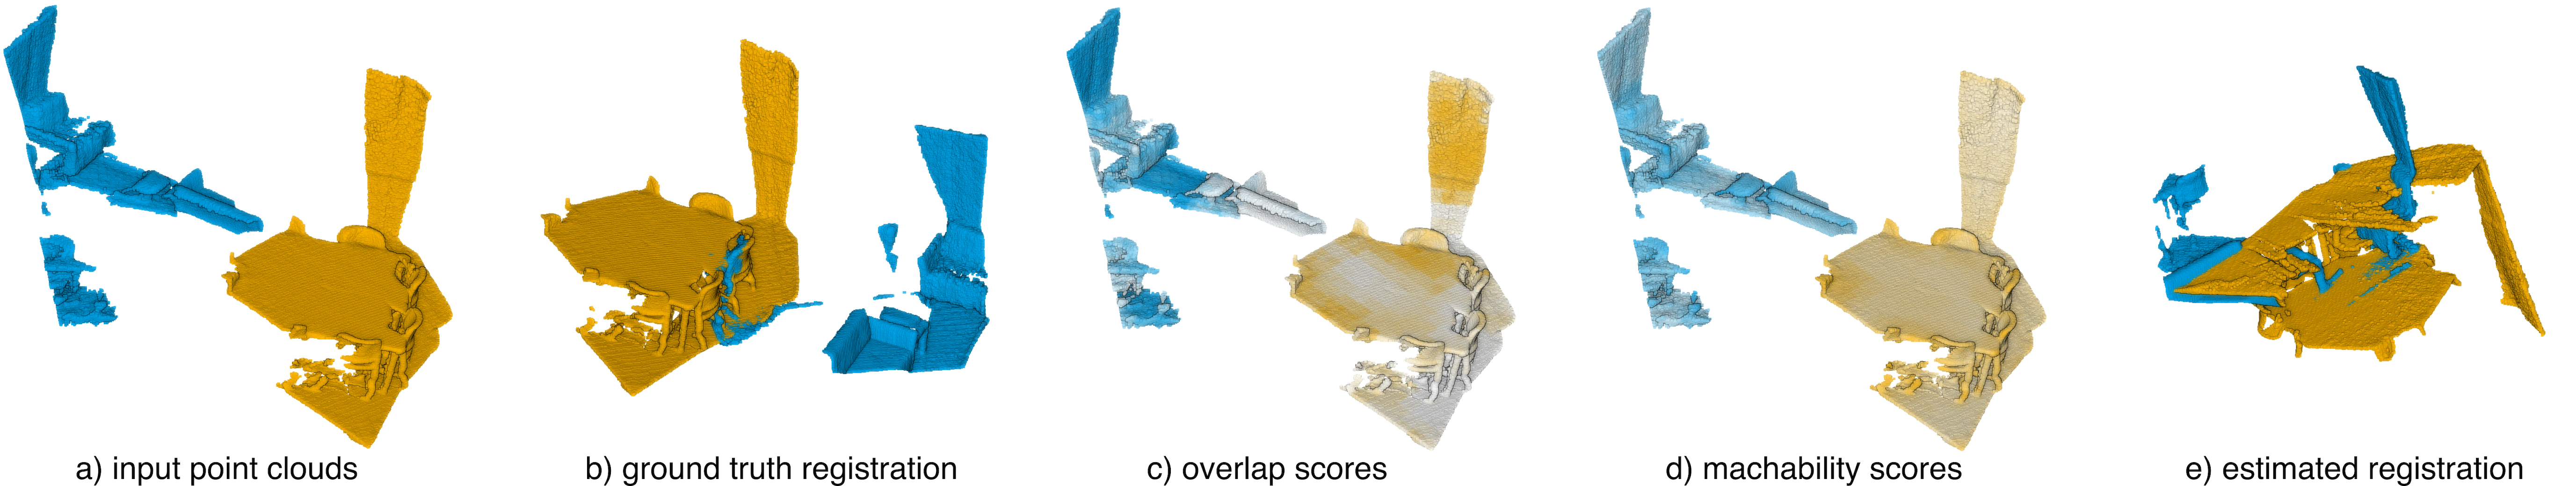
\includegraphics[width=1\columnwidth]{figures/images/one_row.jpg}
    \caption{An extreme case where the overlap is insufficient for registration even with the proposed attention mechanism.}
    \label{fig:failure_image}
\end{figure}
\paragraph{Interest point sampling}
\acro\ significantly increases the effective overlap, but does that improve registration performance?
To test this we use the product of the overlap scores $\mathbf{o}$ and matchability scores $\mathbf{m}$ to bias interest point sampling.
We compare two variants: \emph{top-k (om)}, where we pick the top-$k$ points according to the multiplied scores;
and \emph{prob.\ (om)}, where we instead sample points with probability proportional to the multiplied scores. 

For a more comprehensive assessment we follow~\cite{bai2020d3feat} and report performance with different numbers of sampled interest points. Tab.~\ref{tab:3DMatch_sampling} shows that any of the informed sampling strategies greatly increases the \emph{inlier ratio}, and as a consequence also the \emph{registration recall}.
The gains are larger when fewer points are sampled. In the low-overlap regime the inlier ratios more than triple for up to 1000 points.
We observe that, as expected, high inlier ratio does not necessarily imply high registration recall: our scores are apparently well calibrated, so that \emph{top-k (om)} indeed finds most inliers, but these are often clustered and too close to each other to reliably estimate the transformation parameters (Fig.~\ref{fig:sampling}).
We thus use the more robust \emph{prob. (om)} sampling, which yields the best \emph{registration recall}. It may be possible to achieve even higher registration recall by combining \emph{top-k (om)} sampling with non-maxima suppression. We leave this for future work.

% \begin{table}[t]
%     \setlength{\tabcolsep}{6pt}
%     \renewcommand{\arraystretch}{1.2}
% 	\centering
% 	\resizebox{0.9\columnwidth}{!}{
%     \begin{tabular}{lccccc|ccccc}
% 			\toprule
% 			& \multicolumn{5}{c|}{\textit{3DMatch}} & \multicolumn{5}{c}{\textit{3DLoMatch}} \\
% 			\# Samples & 5000 & 2500 & 1000 & 500 & 250 & 5000 & 2500 & 1000 & 500 & 250 \\
%             \midrule
% 			& \multicolumn{10}{c}{\textit{Registration Recall (\%)}} \\
% 		    \midrule
%  			3DSN~\cite{gojcic20193DSmoothNet} & 78.4 & 76.2 & 71.4 & 67.6 & 50.8 & 33.0 & 29.0 & 23.3 & 17.0 & 11.0  \\
%  			FCGF~\cite{Choy2019FCGF} & \underline{85.1} & \underline{84.7} & 83.3 & 81.6 & 71.4 & \underline{40.1} & 41.7 & 38.2 & 35.4 & 26.8 \\
%  			D3Feat~\cite{bai2020d3feat} & 81.6 & 84.5 & \underline{83.4} & \underline{82.4} & \underline{77.9} & 37.2 & \underline{42.7} & \underline{46.9} & \underline{43.8} & \underline{39.1} \\
%  			\acro\ & \textbf{89.0} & \textbf{89.9} & \textbf{90.6} & \textbf{88.5} & \textbf{86.6} & \textbf{59.8} & \textbf{61.2} & \textbf{62.4} & \textbf{60.8} & \textbf{58.1} \\
% 			\bottomrule
			
% 	\end{tabular}
% 	}
% 	\caption{Results on the \emph{3DMatch} and \emph{3DLoMatch} datasets.}
% 	\label{tab:big_predator}
    
% \end{table}



\begin{table}[t]
    \setlength{\tabcolsep}{6pt}
    \renewcommand{\arraystretch}{1.2}
	\centering
    \begin{tabularx}{\columnwidth}{lYYYYY|YYYYY}
			\toprule
			& \multicolumn{5}{c|}{\textit{3DMatch}} & \multicolumn{5}{c}{\textit{3DLoMatch}} \\
			\# Samples & 5000 & 2500 & 1000 & 500 & 250 & 5000 & 2500 & 1000 & 500 & 250 \\
            \midrule
			& \multicolumn{10}{c}{\textit{Registration Recall (\%)}} \\
		    \midrule
 			3DSN~\cite{gojcic20193DSmoothNet} & 78.4 & 76.2 & 71.4 & 67.6 & 50.8 & 33.0 & 29.0 & 23.3 & 17.0 & 11.0  \\
 			FCGF~\cite{Choy2019FCGF} & \underline{85.1} & \underline{84.7} & 83.3 & 81.6 & 71.4 & \underline{40.1} & 41.7 & 38.2 & 35.4 & 26.8 \\
 			D3Feat~\cite{bai2020d3feat} & 81.6 & 84.5 & \underline{83.4} & \underline{82.4} & \underline{77.9} & 37.2 & \underline{42.7} & \underline{46.9} & \underline{43.8} & \underline{39.1} \\
 			\acro\ & \textbf{89.0} & \textbf{89.9} & \textbf{90.6} & \textbf{88.5} & \textbf{86.6} & \textbf{59.8} & \textbf{61.2} & \textbf{62.4} & \textbf{60.8} & \textbf{58.1} \\
			\bottomrule
	\end{tabularx}
	\caption{Results on the \emph{3DMatch} and \emph{3DLoMatch} datasets.}
	\label{tab:big_predator}
    
\end{table}


\paragraph{Comparison to feature-based methods}
We compare \acro\ to recent feature-based registration methods: 3DSN~\cite{gojcic2018learned}, FCGF~\cite{Choy2019FCGF} and D3Feat~\cite{bai2020d3feat}, see Tab.~\ref{tab:big_predator}. 
Even though \acro\ can not solve all the cases (\cf Fig.~\ref{fig:failure_image}), it greatly outperforms existing methods on the low-overlap \emph{3DLoMatch} dataset, improving registration recall by 15.5-19.7 percent points (pp) over the closest competitor---variously FCGF or 3DFeat. 
Moreover, it also consistently reaches the highest registration recall on standard \emph{3DMatch}, showing that its attention to the overlap pays off even for scans with moderately large overlap.
In line with our motivation, what matters is not so much the choice of descriptors, but finding interest points that lie in the overlap region -- especially if that region is small. 
%Additionally, we show that a larger network (see big\acro\ in Tab.~\ref{tab:big_predator}, with 2$\times$ bigger network width) can further boost the performance.


\paragraph{Comparison to direct registration methods}
We also tried to compare \acro\ to recent methods for direct registration of partial point clouds.
Unfortunately, for both PRNet~\cite{wang2019prnet} and RPM-Net~\cite{yew2020rpm}, training on \emph{3DMatch} failed to converge to reasonable results, as already observed in~\cite{choy2020deep}.
It appears that their feature extraction is specifically tuned to synthetic, object-centric point clouds.
Thus, in a further attempt we replaced the feature extractor of RPM-Net with FCGF.
This brought the registration recall on \emph{3DMatch} to 54.9\%, still far from the
85.1\%  that FCGF features achieve with RANSAC.
We conclude that direct pairwise registration is at this point only suitable for geometrically simple objects in controlled settings like \emph{ModelNet40}.


\begin{table}[t!]
    \setlength{\tabcolsep}{10pt}
    \renewcommand{\arraystretch}{1.2}
	\centering
	\resizebox{\columnwidth}{!}{
    \begin{tabular}{lll|cccccc}
			\toprule
			\multicolumn{3}{c}{overlap attention} & \multicolumn{3}{c}{\textit{3DMatch}} & \multicolumn{3}{c}{\textit{3DLoMatch}} \\
            \cline{4-9}
            \multicolumn{1}{c}{\textit{ov.}} & \multicolumn{1}{c}{\textit{$\times$ov.}} & \multicolumn{1}{c}{\textit{cond.}} & FMR & IR & RR & FMR & IR & RR \\
            \hline
            \multicolumn{1}{c}{}& \multicolumn{1}{c}{} & \multicolumn{1}{c}{} & \underline{96.4} & 39.6 & 82.6 & 72.2 & 14.5 & 38.9\\
            \multicolumn{1}{c}{\ding{51}} & \multicolumn{1}{c}{} & \multicolumn{1}{c}{} & 94.6 & 38.3 & 84.1 & 67.1 & 14.3 & 42.8 \\
            \multicolumn{1}{c}{\ding{51}} & \multicolumn{1}{c}{\ding{51}} & \multicolumn{1}{c}{} & \underline{96.4} & 50.8 & 87.7 & \underline{73.8} & 20.9 & 56.5 \\
            \multicolumn{1}{c}{\ding{51}} & \multicolumn{1}{c}{}  & \multicolumn{1}{c}{\ding{51}} &  95.7 & \underline{52.1} & \underline{88.0} & 72.5 & \underline{21.2} & \underline{57.5} \\
            \multicolumn{1}{c}{\ding{51}} & \multicolumn{1}{c}{\ding{51}} & \multicolumn{1}{c}{\ding{51}} & \textbf{96.7} & \textbf{58.0} & \textbf{89.0} & \textbf{78.6} & \textbf{26.7}& \textbf{59.8} \\
			\bottomrule
	\end{tabular}
	}
	\caption{Ablation of the network architecture. \textit{ov.} denotes upsampling the overlap scores; \textit{cond.} denotes conditioning the bottleneck features on the respective other point cloud; \textit{$\times$ov.} denotes upsampling the cross overlap scores.}
	\label{tab:3DMatch_ablation_w_baseline}
	
\end{table}

\paragraph{Ablations study}
We ablate our overlap attention module in Tab.~\ref{tab:3DMatch_ablation_w_baseline}.
We first compare \acro\ with a baseline model, in which we completely remove the proposed overlap attention module. That baseline, combined with random sampling, achieves the 2\textsuperscript{nd}-highest FMR on both benchmarks, but only reaches 82.6\%, respectively 38.9\% RR.
%; much worse than the other variants that include (at least) the overlap scores. 
%The experiment again confirms that high FMR or IR does not imply high RR, and thus good registration performance. 
By adding the overlap scores, RR increases by 1.5, respectively 3.9 pp on \emph{3DMatch} and \emph{3DLoMatch}. Additionally upsampling conditioned feature scores or cross overlap scores further improves performance, especially on \emph{3DLoMatch}. All three parts combined lead to the best overall performance. For further ablation studies, see Appendix.


\subsection{ModelNet40}
\label{sec:model_net}
\paragraph{Dataset}
~\cite{wu2015ModelNet} contains 12,311 CAD models of man-made objects from 40 different categories. We follow~\cite{yew2020rpm} to use 5,112 samples for training, 1,202 samples for validation, and 1,266 samples for testing. Partial scans are generated following~\cite{yew2020rpm}. In addition to \emph{ModelNet} which has 73.5\% pairwise overlap on average, we generate \emph{ModelLoNet} with lower (53.6\%) average overlap. For more details see Appendix. 

\paragraph{Metrics}
We follow \cite{yew2020rpm} and measure the performance using the \emph{Relative Rotation Error (RRE)} (geodesic distance between estimated and GT rotation matrices), the \emph{Relative Translation Error (RTE)} (Euclidean distance between the estimated and GT translations), and the \emph{Chamfer distance (CD)} between the two registered scans.

\paragraph{Relative overlap ratio} 
\begin{figure}[t]
    \centering
    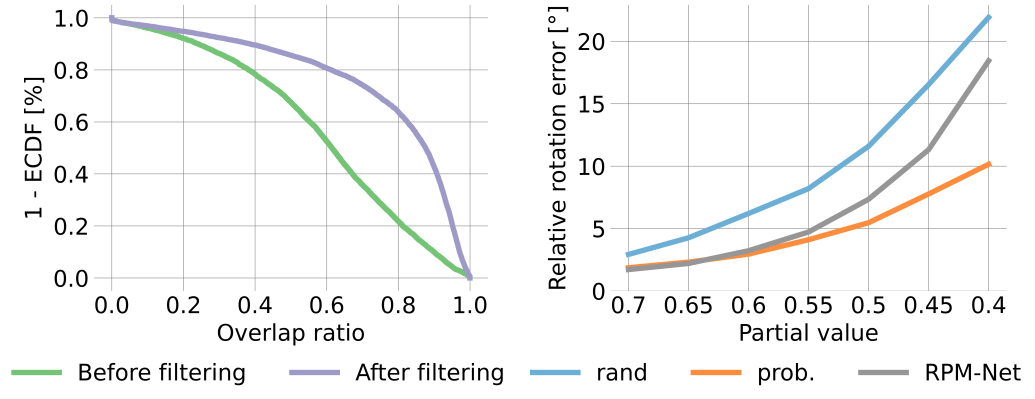
\includegraphics[width=0.8\columnwidth]{figures/images/modelnet.jpg}
    \caption{Improved relative overlap ratio after filtering the points with the inferred overlap scores on 8862 \textit{ModelNet} partial scans(\textit{left}). Owing to the improved overlap ratio, \acro\ is robust to the changes of partial value $p_v$, while the performance of RPM-Net drops rapidly (\textit{right}).  \textit{rand} and \textit{prob.} denote the random and \emph{prob. (om)} biased sampling of 450 interest points, respectively.}%
    \label{fig:modelnet}
    
\end{figure}
We again evaluate if \acro\ focuses on the overlap region. We extract 8,862 test pairs by varying the completeness of the input point clouds from 70 to 40\%. Fig.~\ref{fig:modelnet} shows that \acro\ substantially increases the relative overlap and reduces the number of pairs with overlap \textless70\% by more than 40 pp.

\begin{figure}[t]
    \centering
    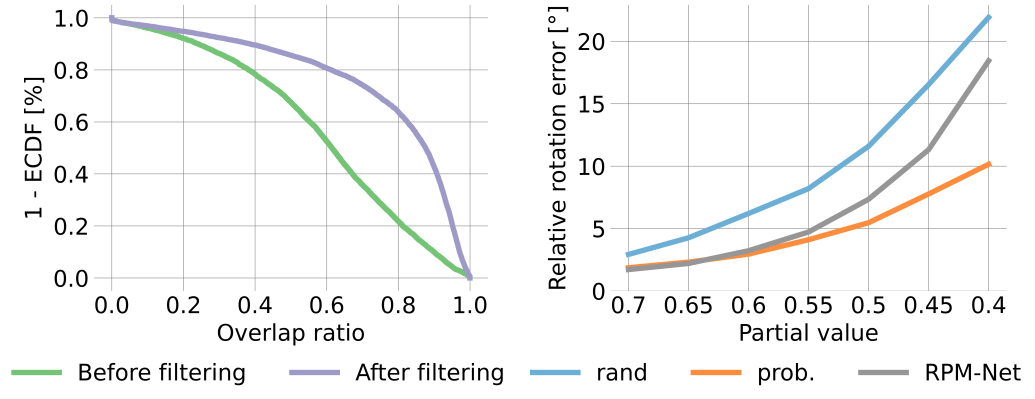
\includegraphics[width=0.8\columnwidth]{figures/images/modelnet.jpg}
    \caption{Improved relative overlap ratio after filtering the points with the inferred overlap scores on 8862 \textit{ModelNet} partial scans(\textit{left}). Owing to the improved overlap ratio, \acro\ is robust to the changes of partial value $p_v$, while the performance of RPM-Net drops rapidly (\textit{right}).  \textit{rand} and \textit{prob.} denote the random and \emph{prob. (om)} biased sampling of 450 interest points, respectively.}%
    \label{fig:modelnet}
    
\end{figure}
\paragraph{Comparison to direct registration methods}
To be able to compare \acro\ to RPM-Net~\cite{yew2020rpm} and DCP~\cite{wang2019dcp}, we resort to the synthetic, object-centric dataset they were designed for. We failed to train PRNet~\cite{wang2019prnet} due to random crashes of the original code (also observed in~\cite{choy2020deep}).
Remarkably, \acro\ can compete with methods specifically tuned for \emph{ModelNet}, and in the low-overlap regime outperforms them in terms of \emph{RRE}, see Tab.~\ref{tab:modelnet}.
Moreover, we observe a large boost by sampling points with overlap attention (\emph{prob.\ (om)}) rather than randomly (\emph{rand}).
Fig.~\ref{fig:modelnet} (right) further underlines the importance of sampling in the overlap: \acro\ is a lot more robust in the low overlap regime ($\approx$8$^\circ$ lower RRE at completeness 0.4). 

\subsection{odometryKITTI}
\label{sec:kitti}
\paragraph{Dataset}
~\cite{geiger2012kitti} contains 11 sequences of LiDAR-scanned outdoor driving scenarios. We follow ~\cite{Choy2019FCGF} and use sequences 0-5 for training, 6-7 for validation, and 8-10 for testing. In line with~\cite{Choy2019FCGF, bai2020d3feat} we further refine the provided ground truth poses using ICP~\cite{besl1992method} and only use point cloud pairs that are at most $10$~m away from each other for evaluation.

\begin{table}[t]
    \setlength{\tabcolsep}{11pt}
    \renewcommand{\arraystretch}{1.05}
	\centering
	\resizebox{\columnwidth}{!}{
    \begin{tabular}{lccccc}
			\hline
			Method & \textit{RTE [cm]}~$\downarrow$ & \textit{RRE [$^\circ$]}~$\downarrow$ & RR~$\uparrow$  \\
			\hline
 			3DFeat-Net~\cite{yew20183dfeat} & 25.9 &  0.57 & 96.0  \\
 			FCGF~\cite{Choy2019FCGF} & 9.5  & 0.30  & 96.6\\
 			D3Feat*~\cite{bai2020d3feat} & \underline{7.2} %
 			& \underline{0.30} %
 			& \textbf{99.8} \\
 			\acro\ (\textit{rand}) & 8.8 & 0.34 & \textbf{99.8}  \\ 
 			\acro\ (\textit{prob. (om)}) &  \textbf{6.8} & \textbf{0.27} & \textbf{99.8} \\
			\hline
	\end{tabular}
	}
	\caption{Evaluation of \acro\ on \emph{odometryKITTI}, following the evaluation protocol employed by D3Feat~\cite{bai2020d3feat}.}
	\label{tab:kitti}
\end{table}
\paragraph{Comparision to the SoTAs}
We compare \acro\ to 3DFeat-Net~\cite{yew20183dfeat}, FCGF~\cite{Choy2019FCGF} and D3Feat*~\cite{bai2020d3feat}\footnote{We find that the released D3Feat code fails to reproduce the results in the paper, possible due to hyper-parameter changes.}
%on \emph{odometryKITTI}. 
As shown in Tab.~\ref{tab:kitti}, \acro\ performs on-par with the SoTA. The results also corroborate the impact of our overlap attention %(\textit{prob.(om)}), 
which again outperforms the random sampling baseline.
%(\textit{rand}). 

\paragraph{Computational complexity}
With $O(n^2)$ complexity the cross-attention module represents the memory bottleneck of \acro. Furthermore, $n$ cannot be selected freely but results from the interplay of (i) the resolution of the initial voxel grid, (ii) the network architecture (number of strided convolution layers), and (iii) the spatial extent of the scene. Nevertheless, by executing the cross-attention at the \emph{superpoint} level, with greatly reduced $n$, we are able to apply \acro\ to large outdoor scans like \emph{odometryKITTI} on a single GPU. For even larger scenes, a simple engineering trick could be to split them into parts, as often done for semantic segmentation.
